\let\negmedspace\undefined
\let\negthickspace\undefined
\documentclass[journal]{IEEEtran}
\usepackage[a5paper, margin=10mm, onecolumn]{geometry}
%\usepackage{lmodern} 
\usepackage{tfrupee} 

\setlength{\headheight}{1cm} 
\setlength{\headsep}{0mm}     

\usepackage{gvv-book}
\usepackage{gvv}
\usepackage{cite}
\usepackage{amsmath,amssymb,amsfonts,amsthm}
\usepackage{algorithmic}
\usepackage{graphicx}
\usepackage{textcomp}
\usepackage{xcolor}
\usepackage{txfonts}
\usepackage{listings}
\usepackage{enumitem}
\usepackage{mathtools}
\usepackage{gensymb}
\usepackage{comment}
\usepackage[breaklinks=true]{hyperref}
\usepackage{tkz-euclide} 
\usepackage{listings}                                        
\def\inputGnumericTable{}                                 
\usepackage[latin1]{inputenc}                                
\usepackage{color}                                            
\usepackage{array}                                            
\usepackage{longtable}                                       
\usepackage{calc}                                             
\usepackage{multirow}                                         
\usepackage{hhline}                                           
\usepackage{ifthen}                                           
\usepackage{lscape}

\begin{document}

\bibliographystyle{IEEEtran}
\vspace{3cm}

\title{4.13.72}
\author{AI25BTECH11003 - Bhavesh Gaikwad}
{\let\newpage\relax\maketitle}

\renewcommand{\thefigure}{\theenumi}
\renewcommand{\thetable}{\theenumi}
\setlength{\intextsep}{10pt} 


\numberwithin{equation}{enumi}
\numberwithin{figure}{enumi}
\renewcommand{\thetable}{\theenumi}


\textbf{Question}: 
A non-zero vector $\vec{a}$ is parallel to the line of intersection of the plane determined by the vectors $\hat{i}, \, \hat{i} + \hat{j}$ and the plane determined by the vectors $\hat{i} - \hat{j}, \, \hat{i} + \hat{k}$. The angle between $\vec{a}$ and the vector $\hat{i} - 2\hat{j} + 2\hat{k}$ is \_\_\_\_\_\_.

\hfill{(1996)}

\textbf{Solution:}\\
Let $\vec{A}=\myvec{1 \\ 0 \\0}$, $\vec{B}=\myvec{1 \\ 1 \\ 0}$, $\vec{C}=\myvec{1 \\ -1 \\ 0}$ and $\vec{D}=\myvec{1 \\ 0 \\ 1}$\\

\begin{equation}
\text{Let the Equation of Plane-1 be: } \vec{n}^\top\vec{x}=0
\end{equation}

Since $\vec{A}$ and $\vec{B}$ satisfy Equation 0.1,
\begin{equation}
    \vec{n}^\top\vec{A}=0 \text{ And } \vec{n}^\top\vec{B}=0
\end{equation}

\begin{center}
    OR
\end{center}

\begin{equation}
    \vec{A}^\top\vec{n}=0 \text{ And } \vec{B}^\top\vec{n}=0
\end{equation}

From Equation 0.3,
\begin{equation}
    \myvec{\vec{A} & \vec{B}}^\top \vec{n} = 0
\end{equation}

\begin{equation}
    \myvec{ 1 & 0 & 0 \\ 1 & 1 & 0} \vec{n}= 0
\end{equation}

\begin{equation}
    \therefore \, \, \vec{n} = \myvec{0 \\ 0 \\ 1}
\end{equation}
\begin{equation}
    \text{Therefore, The Equation of Plane-1 is } \myvec{0 & 0 & 1}\vec{x} = 0
\end{equation}


\begin{equation}
\text{Let the Equation of Plane-2 be: } \vec{m}^\top\vec{x}=0
\end{equation}

Since $\vec{C}$ and $\vec{D}$ satisfy Equation 0.8,
\begin{equation}
    \vec{m}^\top\vec{C}=0 \text{ And } \vec{n}^\top\vec{D}=0
\end{equation}

\begin{center}
    OR
\end{center}

\begin{equation}
    \vec{C}^\top\vec{m}=0 \text{ And } \vec{D}^\top\vec{m}=0
\end{equation}

From Equation 0.10,
\begin{equation}
    \myvec{\vec{C} & \vec{D}}^\top \vec{m} = 0
\end{equation}

\begin{equation}
    \myvec{ 1 & -1 & 0 \\ 1 & 0 & 1} \vec{m}= 0
\end{equation}

\begin{equation}
    \therefore \, \, \vec{m} = \myvec{1 \\ 1 \\ -1}
\end{equation}
\begin{equation}
    \text{Therefore, The Equation of Plane-2 is } \myvec{1 & 1 & -1}\vec{x} = 0
\end{equation}\\\\

Let the parallel vector of line of intersection of Plane-1 and Plane-2 be $\vec{r}$.\\

As $\vec{r}$ satisfies the Equation of both the Planes,
\begin{equation}
    \vec{n}^\top\vec{r}=0 \, \, \& \, \, \vec{m}^\top\vec{r}=0
\end{equation}

From Equation 0.15,
\begin{equation}
    \myvec{\vec{n} & \vec{m}}^\top\vec{r}=0
\end{equation}

\begin{equation}
\myvec{ 0 & 0 & 1 \\ 1 & 1 & -1}\vec{r}  =0
\end{equation}

\begin{equation}
    \therefore \, \, \vec{r} = \myvec{ 1 \\ -1 \\ 0}
\end{equation}


\begin{equation}
\text{Therefore from Equation 0.18, } \vec{a} = \myvec{1 \\ -1 \\ 0}    
\end{equation}

Let $\vec{u} = \myvec{1 \\ -2 \\ 2}$ $\quad$ [Already given in the Question]\\

We know,
\begin{equation}
    \vec{a}^\top\vec{u} = \norm{\vec{a}}\norm{\vec{u}}\cos(\theta)
\end{equation}

\begin{equation}
    \norm{\vec{a}} = \sqrt{\vec{a}^\top\vec{a}} = \sqrt{2}, \, \norm{\vec{u}} = \sqrt{\vec{u}^\top\vec{u}} = 3
\end{equation}\\

From Equation 0.20 and 0.21,
\begin{equation}
    \cos(\theta) = \dfrac{3}{3\sqrt{2}} \quad \Rightarrow \theta = 45^\circ
\end{equation}

\begin{align}
  \boxed{\text{The angle between } \vec{a} \text{ and } 1\hat{i} -2\hat{j}+2\hat{k} \text{ is } 45^{\circ}.}  
\end{align}

\begin{figure}[htbp]
    \centering
    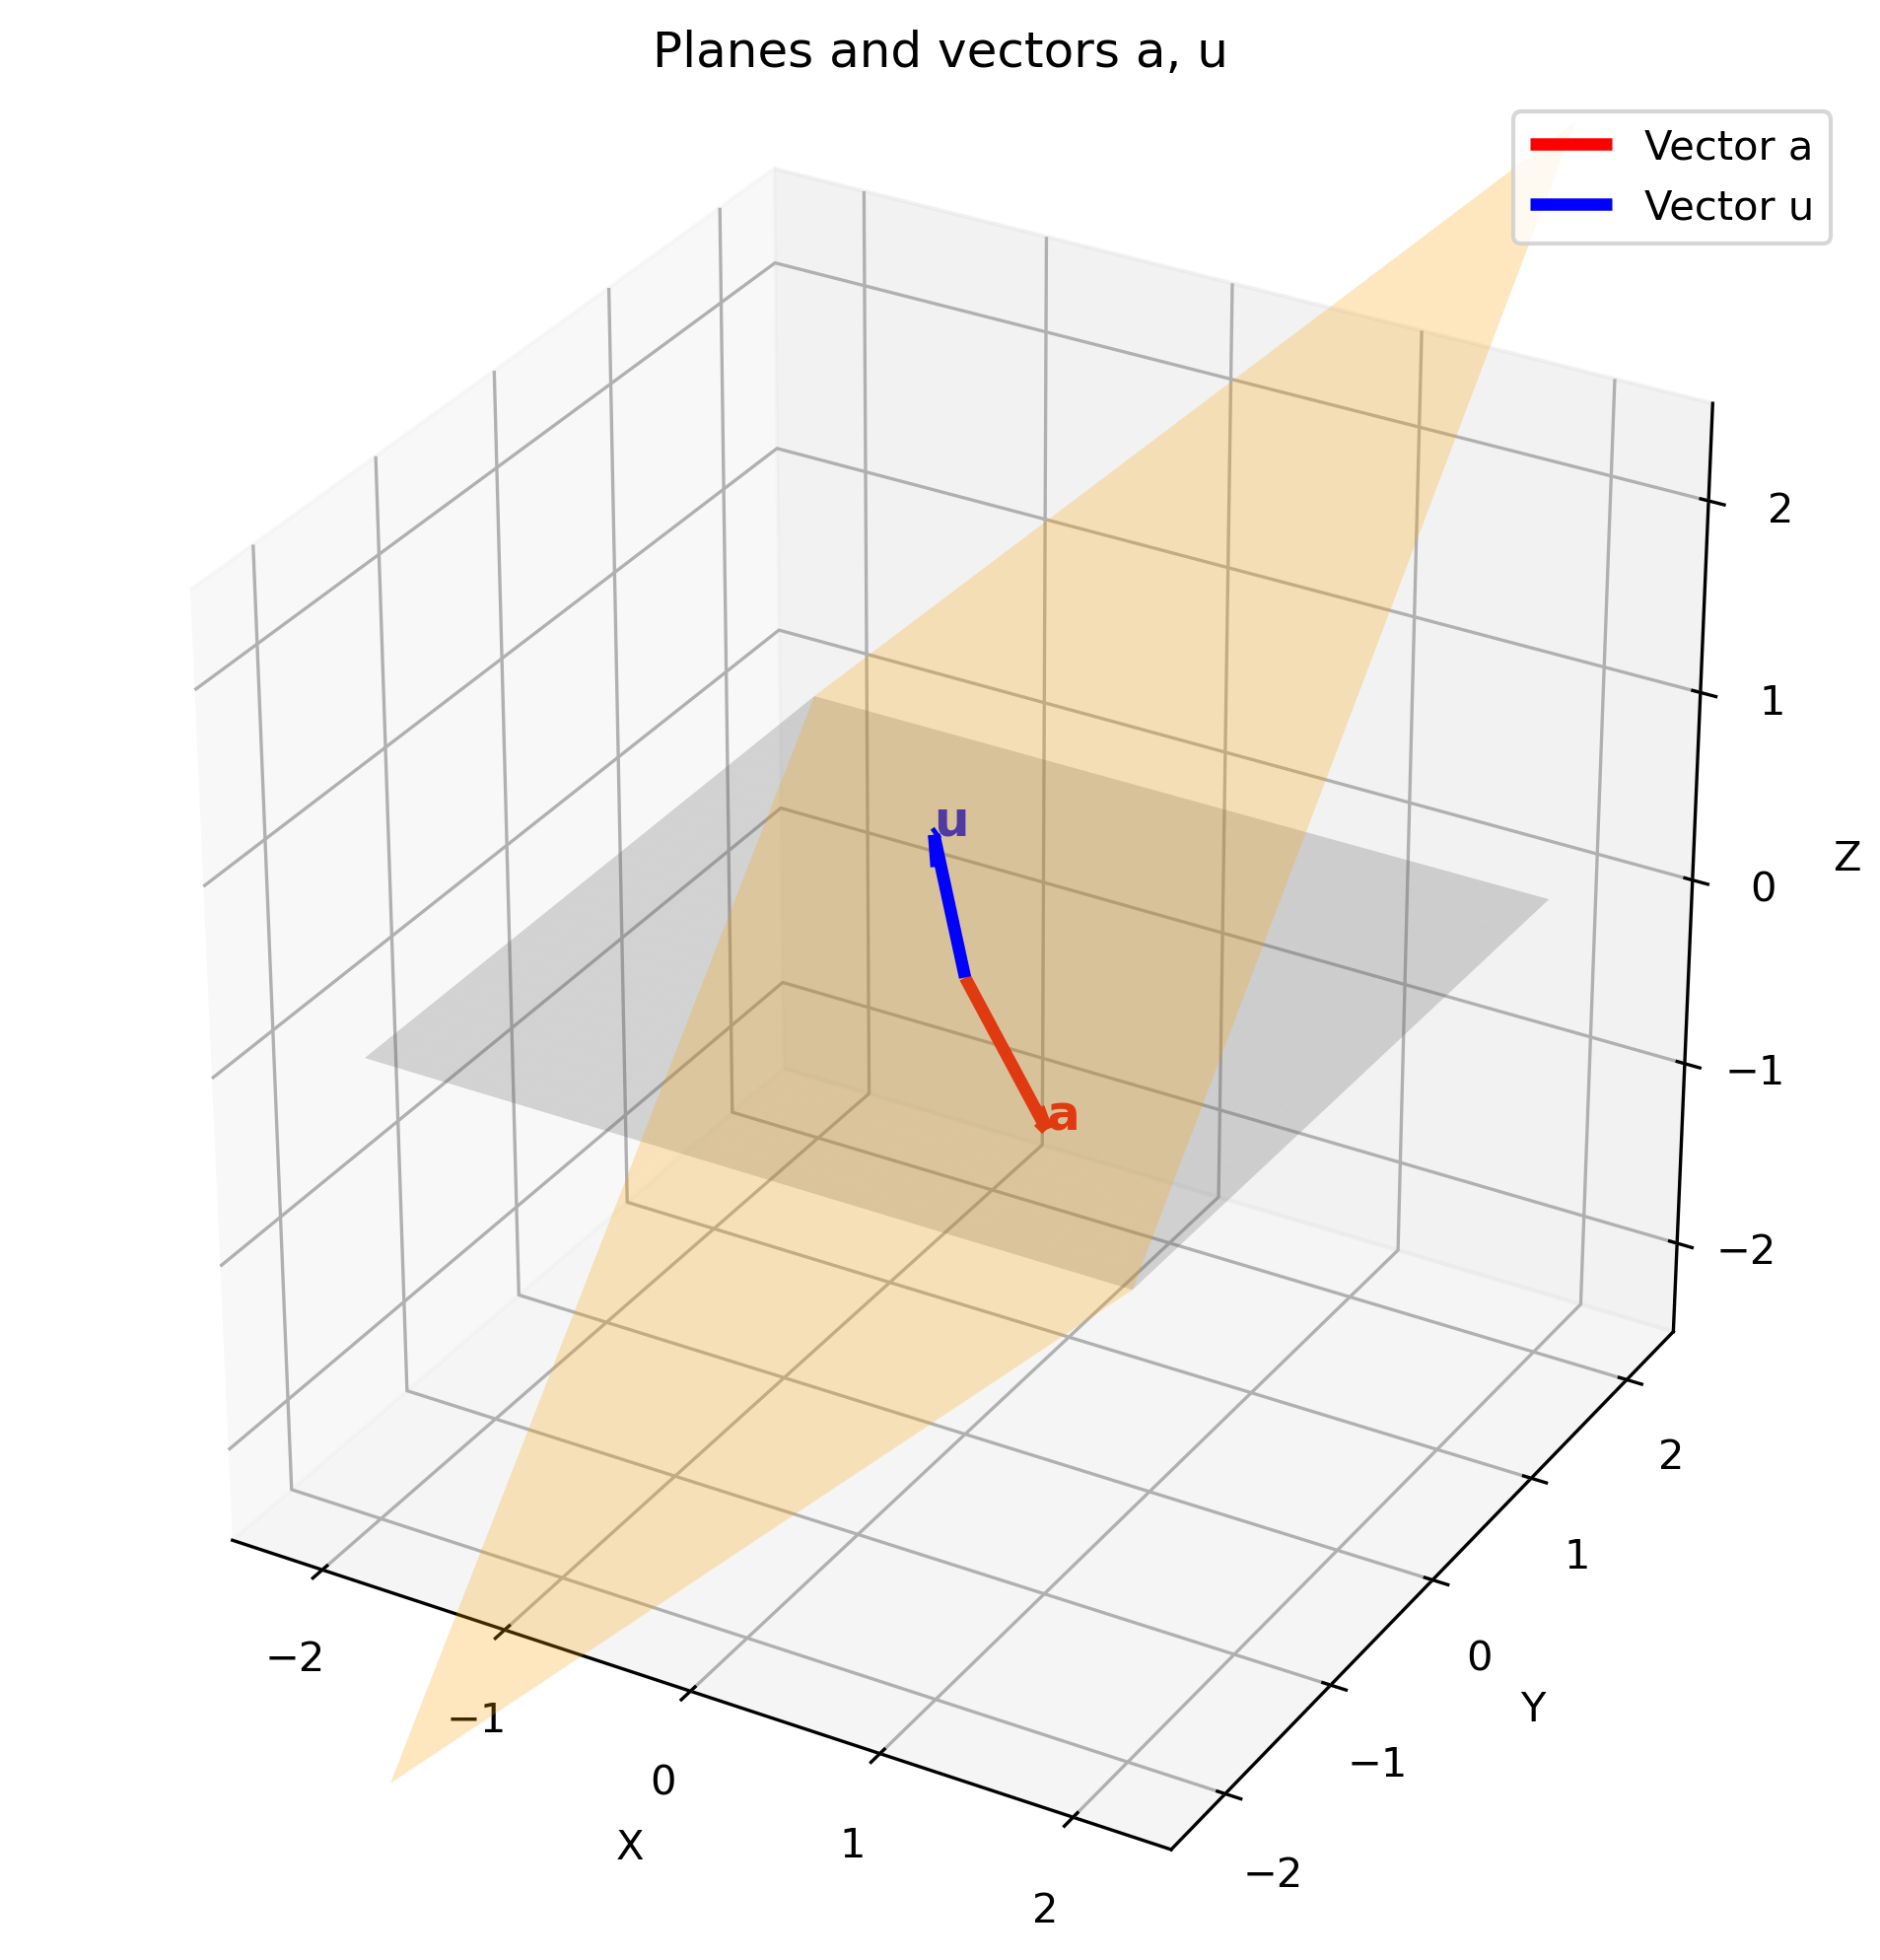
\includegraphics[width=\columnwidth]{figs/fig1.png}
    \caption{Plane}
    \label{fig:fig/fig1.png}
\end{figure}
\end{document}  
